
\documentclass[conference]{IEEEtran}
\usepackage [english]{babel}
\usepackage [autostyle, english = american]{csquotes}
\usepackage[rightcaption]{sidecap}
\usepackage{graphicx} %package to manage images
\graphicspath{ {images/} }

\usepackage[font=bf]{caption}
\usepackage{subcaption}
\MakeOuterQuote{"}

\begin{document}
\title{\LARGE Predicting and Removing Non-Analogous Data in a Genetic Algorithm \\ \large [Mitigating Erroneous Patterns by Analyzing the Regression Effect produced by Outliers]}

% author names and affiliations
% use a multiple column layout for up to three different
% affiliations
\author{\IEEEauthorblockN{Taylor Ripke}
\IEEEauthorblockA{Central Michigan University\\
Mount Pleasant, MI 48859\\
Email: ripke1tj@cmich.edu}
\and
\IEEEauthorblockN{Jacob Fishbaugh}
\IEEEauthorblockA{Central Michigan University\\
Mount Pleasant, MI 48859\\
Email: fishb1jw@cmich.edu}
\and
\IEEEauthorblockN{Kellen Reason\\}
\IEEEauthorblockA{Central Michigan University\\
Mount Pleasant, MI 48859\\
Email: reaso1km@cmich.edu}}

% conference papers do not typically use \thanks and this command
% is locked out in conference mode. If really needed, such as for
% the acknowledgment of grants, issue a \IEEEoverridecommandlockouts
% after \documentclass

% for over three affiliations, or if they all won't fit within the width
% of the page, use this alternative format:
% 
%\author{\IEEEauthorblockN{Michael Shell\IEEEauthorrefmark{1},
%Homer Simpson\IEEEauthorrefmark{2},
%James Kirk\IEEEauthorrefmark{3}, 
%Montgomery Scott\IEEEauthorrefmark{3} and
%Eldon Tyrell\IEEEauthorrefmark{4}}
%\IEEEauthorblockA{\IEEEauthorrefmark{1}School of Electrical and Computer Engineering\\
%Georgia Institute of Technology,
%Atlanta, Georgia 30332--0250\\ Email: see http://www.michaelshell.org/contact.html}
%\IEEEauthorblockA{\IEEEauthorrefmark{2}Twentieth Century Fox, Springfield, USA\\
%Email: homer@thesimpsons.com}
%\IEEEauthorblockA{\IEEEauthorrefmark{3}Starfleet Academy, San Francisco, California 96678-2391\\
%Telephone: (800) 555--1212, Fax: (888) 555--1212}
%\IEEEauthorblockA{\IEEEauthorrefmark{4}Tyrell Inc., 123 Replicant Street, Los Angeles, California 90210--4321}}




% use for special paper notices
%\IEEEspecialpapernotice{(Invited Paper)}




% make the title area
\maketitle


\begin{abstract}
Genetic algorithms mimic the process of natural selection and have been proven to solve complex problems. Given a population, the algorithm mates random chromosomes based on the fitness level which in turn produces a better generation. Based on information present in our system, an adaptive genetic algorithm compute the necessary calories needed to burn fat, future PR’s, and weight lifts. However, non-analogous data within the initial pool can alter the results. Therefore, it is necessary to predict this data and remove it to produce the best possible outcome. In this paper, we present a genetic algorithm that predicts invalid data by comparing it to other data present in the pool and removes it in hopes of raising the solutions fitness to exceed the results predicted by an unmodified genetic algorithm. We report the results of the program used to test this modified approach. Our preliminary results show a 7.2ms increase in performance using the modified genetic algorithm. We believe that the results could be improved with further optimization and that the effects of this algorithm are more applicable on a larger scale. 

\blindtext[1]
\end{abstract}
% IEEEtran.cls defaults to using nonbold math in the Abstract.
% This preserves the distinction between vectors and scalars. However,
% if the journal you are submitting to favors bold math in the abstract,
% then you can use LaTeX's standard command \boldmath at the very start
% of the abstract to achieve this. Many IEEE journals frown on math
% in the abstract anyway.

% Note that keywords are not normally used for peerreview papers.
\begin{IEEEkeywords}
Genetic Algorithm, Mutation
\end{IEEEkeywords}






% For peer review papers, you can put extra information on the cover
% page as needed:
% \ifCLASSOPTIONpeerreview
% \begin{center} \bfseries EDICS Category: 3-BBND \end{center}
% \fi
%
% For peerreview papers, this IEEEtran command inserts a page break and
% creates the second title. It will be ignored for other modes.
\IEEEpeerreviewmaketitle

\large 1. Introduction

Outliers may be classified among several definitions, but a consensual definition is that they are data that lies outside the threshold of the general population. Although the varying degree with which they will affect the outcome is constrained to the given situation, in most cases, they will alter the results slightly. Other approaches to outlier detection and removal have proved successful and demonstrate exceptional outlier removal. The approach that we propose demonstrates similar results, with a strong emphasis on how the outliers are removed. The proposed algorithm traverses the given data set looking for patterns and considers each outlier before removal.

For our project, we will be creating a modified genetic algorithm that will remove outliers before computing in order to reduce CPU time and improve the group of solutions previously given by an unmodified genetic algorithm. The algorithm that removes these outliers will be key to our research as we hope to increase the efficiency of the genetic algorithm by at least 10 times to exceed the results by others researchers in this area. We will be creating the modified genetic algorithm from scratch and modifying it to fit our needs. Once the modified genetic algorithm is complete, we will be testing it against an unmodified genetic algorithm with the outliers present to show the increase in efficiency and accuracy of the predication made. Our genetic algorithm will be predicting the amount of calories needed to burn and the weight you can lift based on previous data entries in the database. We hope to find two things as a result of this research project: The modified genetic algorithm proves to be more efficient that the unmodified genetic algorithm during testing and that the method using to extract the outliers from the data set is more efficient than previous work in the field. 

We begin with an in-depth look at prior work in the field and use that as a basis for our research. Next, we describe our methodology and approach taken. The results are presented in the discussion section and plans for future work are also outlined. 



\large 2. Background and Related Work

\large Given a random population, the purpose of a genetic algorithm is to solve a complex task by mimicking the process of natural selection in nature. From the population, a score is given to each member. This score determines how likely that element will be chosen when it is time to mate two parents based on its fitness. Children are produced from the parents who are used to form the next generation. However, one area of interest is in the removal of non-analogous data from the initial generation, hopefully producing a better result and increasing the solutions fitness. For example, if given information such as how much weight a person has lifted while exercising, it is important to remove information that may affect the progress or result of the algorithm. If a person is lifting weight of 135 pounds consecutively and is steadily increasing 5 to 10 pounds every week, a data entry of 65 pounds will influence the calculation because it makes little sense that there would be a steep decrease for no reason. Therefore, the purpose of this modified genetic algorithm is to analyze the data before running the calculations, remove the non-analogous data, and perform the calculations. By removing this data, we hope to get a more efficient algorithm with more accurate results. 

\large Each population the genetic algorithm runs through is calculated and produced when two parents mate to form children. Although a few instances may not affect the model, if the data scanned is for a sufficient period of time and there are many instances, this non-analogous data may affect the outcome of the genetic algorithm. Each chromosome is given a fitness value based on how close it is to the fitness function of where the algorithm thinks that it should be at. Entities with a higher fitness are more likely to be chosen as it is a higher value. It is possible, however, that a chromosome with a low fitness value may be chosen, because it is truly random and there needs to be diversity in the calculations. Moreover, if there are many instances of non-analogous data and if they are chosen, it will take longer for the genetic algorithm to find the maximum fitness solution because it will have to run more generations due to many instances of incorrect values.  


2.1 Lanzi et al.


\large Although not the same idea, a similar approach was taken by Lanzi where he used filters for fast features selection using a genetic algorithm. Given a dataset with n attributes, the goal was to find the minimum number of m relevant attributes to describe the data. He noted that previous approaches using genetic algorithms analyzed all data of a dataset and required large amounts of CPU time to reach a good solution on a large dataset. The results of his algorithm showed that it required overall less CPU time to reach a relevant subset of features for his image selection. He also showed that his genetic algorithm for feature selection was at least 10 times faster than a standard genetic algorithm using all data. The modified algorithm showed no loss of predictive accuracy when the learning algorithm he devised was applied to his reduced dataset [1]. 

\large This idea employs a similar set of techniques that we want to employ to our dataset. Lanzi showed that for image selection, his algorithm was able to find features more quickly using a modified genetic algorithm on a restricted dataset rather than using all data present. One of the differences between our research is that all the data that he is using is relevant to his research. He is trying to find ways to reduce the computational load that his CPU must do by reducing the amount of data that needs to be processed. Our research is focused on removing non-analogous data from the dataset before the computations are performed to not only reduced computation time in the CPU, but also try to increase the algorithms results. 

2.2 Nahum et al.

\large Similar work has also been conducted by Nahum et al.  where they produced a multi-objective genetic algorithm for outlier removal. In their research, the acknowledge that the presence of outliers can compromise the ability of statistical methods producing mediocre prediction statistics. Therefore, it is important to remove these outliers before running the algorithm. The algorithm presented in their research removes these outliers by comparing adjacent data and calculating the difference between them. If it exceeds a specific threshold, the data is removed from the calculation. The research that we want to conduct will be to suggest a new algorithm for the detection of outliers and prove its efficiency against other models that perform a similar task. 

\large Adaptive Probabilities of Crossover and Mutation in Genetic Algorithms discusses a notion of an adaptive genetic algorithm that targets generational replacement, whereby the best solutions are explicitly protected from disruption and adapting the mutation and crossover based on fitness values. As opposed to most implementations of genetic algorithms where the mutation level is varied in a predetermined fashion or the operator probabilities are invariant with the individual finesses of solutions. The adaptive genetic algorithm required the modification of the popularly used Schema theorem, which provides the building blocks that form the solutions. The Schema theorem is able to form solutions by predicting the growth of high fitness building blocks at the expense of low fitness ones. The author proposes a way to derive the Schema theorem for the genetic algorithm with adaptive crossover and mutation values. Most importantly, the adaptive genetic algorithm produces an approach that prevents the convergence of a typical genetic algorithm to a local optimum.

\large These solutions produced by the Schema theorem favor the prediction of higher building blocks which produce more accurate results at the expense of the low fitness ones. By removing the outliers, the adaptive genetic algorithm can prevent an early convergence, but hopefully bring about the answer much quickly that a typical genetic algorithm. We will be expanding upon previous research that has been done in the field and we will be suggesting a modified genetic algorithm that efficiently analyzes that data before execution, removing the non-analogous data to produce optimal results. 

3. Method

3.1 Overview of Existing Systems

Outliers within a given dataset can obscure or delay the results of a genetic algorithm. The genetic algorithm analyzes the fitness of each chromosome with respect to the goal. The chromosomes with a higher fitness are more likely to be selected to be present within the next population. However, genetic diversity is necessary in nature for a species to evolve and survive. Therefore, variations in data are necessary; however, the extreme to which they are present can be controlled to improve efficiency.

As discussed previously, Lanzi et al. applied a similar technique where they found the minimum number of relevant attributes necessary to describe the data they were using. In their research, they acknowledged that utilizing all of the data in the dataset required large amounts of CPU utilization to reach an acceptable result. Rather, the approach only utilized the necessary attributes and they were able to run their genetic algorithm at least 10 times faster than the standard genetic algorithm without losing any accuracy. Lanzi et al. is focused on removing the computational load needed to be done. All of the data present in their study is important to their research. Our research is primarily focused on removing the non-analogous data from the data set before the computations are performed.

Genetic Algorithms are learning programs and they learn how to do a certain task over time. One key feature that genetic algorithms provide is variation. Therefore, they can be used to find different ways of arriving at the same goal. For example, for someone who is on a training regime, a genetic algorithm could develop a training plan for them to follow to help them reach their specific goals. If the athlete does not like the workout presented, a genetic algorithm could regenerate a workout that still meets the needs of the athletes, but in a different way. A genetic algorithm could do this by using previously entered data to predict future training regimes. However, the presence of outliers could affect the outcome of the genetic algorithm in several ways. Outliers can delay the generation and accuracy of data. A dataset with many outliers may take longer to complete and the results may be less accurate than a dataset without. Our research proposes a new algorithm to remove outliers from a dataset before calculation to ensure improved accuracy and efficiency. 

Specifically, our research will focus on developing a smart outlier removal algorithm. An outlier is considered any data that does not relate to other data present. This can be computed by taking the average of the dataset, for example, and determining a threshold. The threshold is a specific condition that the data cannot go above or below. If it is outside those bounds, it is considered an outlier and is subject for removal. However, not all non-analogous data is to be removed as it may be there for a reason. Therefore, we need to develop a smart outlier removal algorithm to handle these situations which are discussed below. 

3.2 Proposed System

For the purposes of this experiment, we created a modified genetic algorithm that removes outliers in the initial population. The results of our experiment were produced by comparing the modified genetic algorithm to an unmodified genetic algorithm to see which was more efficient. The task of the genetic algorithm was to find four numbers that added up to a specific target value. A constraint was placed on the numbers that they must be between a certain range. If the numbers were outside a specific threshold, they were removed from the initial population from which the genetic algorithm ran its generations. 

3.2.1 Modified Genetic Algorithm

The modified genetic algorithm had an additional method which removed the outliers from a given population before the generations were produced. The algorithm works by first calculating a given threshold based on the initial data and constraints placed on the values computed to produced a computed average. From the average, the threshold was computed by evaluating distance between the lowest and highest value in the data set. At this point, it would have been easy to remove the outliers from the dataset, but it is important to consider the ramifications this would have if the data outside the given threshold was important to the overall system. Refer to figure 1.0.

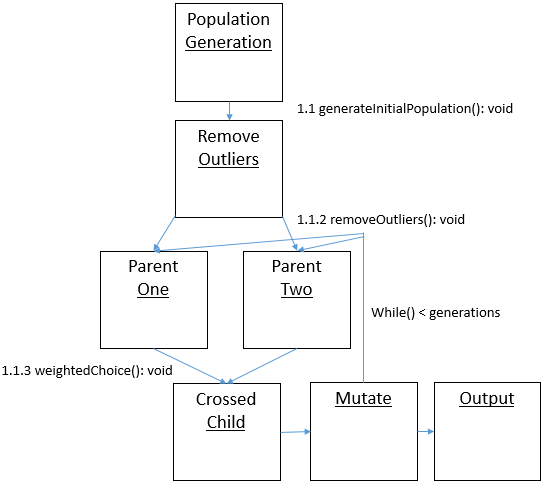
\includegraphics[scale=0.5]{Collab}
Figure 1.0


Therefore, the next stage of the algorithm determines the frequency of the outliers, specifically looking for any pattern present in the data. For example, if there was always a specific value on this day of the week over a given period of time, we know that this data is most likely important and should not be removed from the calculation. However, if the outliers present in the data appear to be random, they can most likely be removed. 

Another factor we considered during the development of this algorithm was predicting growth change. For example, if an athlete is consecutively making progress, we should expect the weight they are lifting to remain the same or steadily increase. However, if in the data set the values suddenly drop and remain at this new value, we know something must have happened ie. the athlete may have been injured. The genetic algorithm must be able to accommodate to changes in data over time and modify the end result.

As stated previously, a genetic algorithm relies on diversity to achieve the highest fitness. Therefore, it is also necessary to compute the difference between outliers and determine which of them have more relevance. We can do this by computing the difference in their values and comparing them to the average of the data set. Outliers further away from the average will not be included in the initial population; however, more relevant ones will for genetic diversity. 

To ensure that each outlier is considered before removal, we compare subsections of the dataset with others to consider the effect they have. Given some subsection, we can compute the average of it and compare it to the average of another subsection. This will lower the rating of the outliers that produce an average farther away from the global average. Finally, once these calculations are complete, we traverse the initial population and remove the flagged outliers.

3.2.2 Implementation

The preliminary scans check the population for outliers and then adds them to an ArrayList for further processing. In a method called CheckOutliers, the outliers are checked for patterns and returns a fitness value for them. If the outliers surpass the fitness value, they will be excluded from the population. However, if they do not, they will be considered in the initial population.

Once the outliers have been removed from the population, the genetic algorithm is run and the efficiency of it is recorded. The results are then compared with the unmodified genetic algorithm with the outliers present. The results, as shown below, display that the removal of non-analogous data from the data set increase the performance slightly. Given a bigger population and generation set, we believe these results could be improved further. 


3.2.3 Results

Following the successful implementation of the modified genetic algorithm, we were able to find a positive trend among the modified genetic algorithm. In comparison to the unmodified genetic algorithm, we found with our initial population that the algorithm ran an average of 7.2ms faster. The initial population was 100 and we ran 1000 generations of this algorithm, producing optimal results each time. The algorithm's efficiency was computed while the generations were being computed. The time take to remove outliers from the initial population was not considered as we were primarily focused on the efficiency of the generations. 

As shown in the results section, the modified genetic algorithm outperformed its unmodified counterpart. The improved performance is a direct result of removing the non-analogous values from the initial data set. Consistent with removing outlying data members, the modified genetic algorithm was able to produce an increased fitness solution causing a greater propagation efficiency.

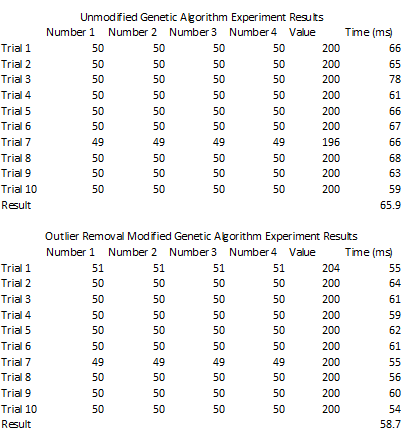
\includegraphics[scale=0.8]{GA}
Figure 2.0

\large 5. Conclusion

As shown in figure 2.0, both genetic algorithms produced the same results each time. However, the modified genetic algorithm outperformed the unmodified genetic algorithm over a series of tests. With further modification, we believe that given a larger data set, the results would improve even more. The approach employed in this system utilizes a similar, yet different approach than other systems in existence, approach and produces favorable results. 

In the future, we plan to take a more extensive approach and build upon our existing system to further increase efficiency. A neural network will be developed using correct data and the neural network will be used to determine the relevance of any given member in the population. This approach will be a more sophisticated method than we previously used as it can make decisions based on other data in the field, rather than arbitrary checks.  
% needed in second column of first page if using \IEEEpubid
%\IEEEpubidadjcol

% An example of a floating figure using the graphicx package.
% Note that \label must occur AFTER (or within) \caption.
% For figures, \caption should occur after the \includegraphics.
% Note that IEEEtran v1.7 and later has special internal code that
% is designed to preserve the operation of \label within \caption
% even when the captionsoff option is in effect. However, because
% of issues like this, it may be the safest practice to put all your
% \label just after \caption rather than within \caption{}.
%
% Reminder: the "draftcls" or "draftclsnofoot", not "draft", class
% option should be used if it is desired that the figures are to be
% displayed while in draft mode.
%
%\begin{figure}[!t]
%\centering
%\includegraphics[width=2.5in]{myfigure}
% where an .eps filename suffix will be assumed under latex, 
% and a .pdf suffix will be assumed for pdflatex; or what has been declared
% via \DeclareGraphicsExtensions.
%\caption{Simulation Results}
%\label{fig_sim}
%\end{figure}

% Note that IEEE typically puts floats only at the top, even when this
% results in a large percentage of a column being occupied by floats.


% An example of a double column floating figure using two subfigures.
% (The subfig.sty package must be loaded for this to work.)
% The subfigure \label commands are set within each subfloat command, the
% \label for the overall figure must come after \caption.
% \hfil must be used as a separator to get equal spacing.
% The subfigure.sty package works much the same way, except \subfigure is
% used instead of \subfloat.
%
%\begin{figure*}[!t]
%\centerline{\subfloat[Case I]\includegraphics[width=2.5in]{subfigcase1}%
%\label{fig_first_case}}
%\hfil
%\subfloat[Case II]{\includegraphics[width=2.5in]{subfigcase2}%
%\label{fig_second_case}}}
%\caption{Simulation results}
%\label{fig_sim}
%\end{figure*}
%
% Note that often IEEE papers with subfigures do not employ subfigure
% captions (using the optional argument to \subfloat), but instead will
% reference/describe all of them (a), (b), etc., within the main caption.


% An example of a floating table. Note that, for IEEE style tables, the 
% \caption command should come BEFORE the table. Table text will default to
% \footnotesize as IEEE normally uses this smaller font for tables.
% The \label must come after \caption as always.
%
%\begin{table}[!t]
%% increase table row spacing, adjust to taste
%\renewcommand{\arraystretch}{1.3}
% if using array.sty, it might be a good idea to tweak the value of
% \extrarowheight as needed to properly center the text within the cells
%\caption{An Example of a Table}
%\label{table_example}
%\centering
%% Some packages, such as MDW tools, offer better commands for making tables
%% than the plain LaTeX2e tabular which is used here.
%\begin{tabular}{|c||c|}
%\hline
%One & Two\\
%\hline
%Three & Four\\
%\hline
%\end{tabular}
%\end{table}


% Note that IEEE does not put floats in the very first column - or typically
% anywhere on the first page for that matter. Also, in-text middle ("here")
% positioning is not used. Most IEEE journals use top floats exclusively.
% Note that, LaTeX2e, unlike IEEE journals, places footnotes above bottom
% floats. This can be corrected via the \fnbelowfloat command of the
% stfloats package.


% if have a single appendix:
%\appendix[Proof of the Zonklar Equations]
% or
%\appendix  % for no appendix heading
% do not use \section anymore after \appendix, only \section*
% is possibly needed

% use appendices with more than one appendix
% then use \section to start each appendix
% you must declare a \section before using any
% \subsection or using \label (\appendices by itself
% starts a section numbered zero.)
%


\appendices


% use section* for acknowledgement


% Can use something like this to put references on a page
% by themselves when using endfloat and the captionsoff option.
\ifCLASSOPTIONcaptionsoff
  \newpage
\fi



% trigger a \newpage just before the given reference
% number - used to balance the columns on the last page
% adjust value as needed - may need to be readjusted if
% the document is modified later
%\IEEEtriggeratref{8}
% The "triggered" command can be changed if desired:
%\IEEEtriggercmd{\enlargethispage{-5in}}

% references section

% can use a bibliography generated by BibTeX as a .bbl file
% BibTeX documentation can be easily obtained at:
% http://www.ctan.org/tex-archive/biblio/bibtex/contrib/doc/
% The IEEEtran BibTeX style support page is at:
% http://www.michaelshell.org/tex/ieeetran/bibtex/
%\bibliographystyle{IEEEtran}
% argument is your BibTeX string definitions and bibliography database(s)
%\bibliography{IEEEabrv,../bib/paper}
%
% <OR> manually copy in the resultant .bbl file
% set second argument of \begin to the number of references
% (used to reserve space for the reference number labels box)
\begin{thebibliography}{1}

\bibitem{IEEEhowto:kopka}
Pier Luca Lanzi, \emph{Fast Feature Selection with Genetic Algorithms: A Filter Approach \LaTeX}, Ponzio 34, I-20133\hskip \relax Milano Italia.

\bibitem{IEEEhowto:kopka1}
Nahum, O. E., Yosipof, A., and Senderowitz, H., \emph{A Multi-Objective Genetic Algorithm for Outlier Removal \LaTeX}, Journal of Chemical Information and Modeling\hskip \relax Irael.

\bibitem{IEEEhowto:kopka2}
Srinivas, M., Patnaik, L.M., \emph{Adaptive Probablilites of Crossover and Mutation in Genetic Algorithms \LaTeX}, IEEE Transactions on systems, man and cyvernetics Vol 34. No. 4 April 1994.\hskip \relax

\end{thebibliography}

% biography section
% 
% If you have an EPS/PDF photo (graphicx package needed) extra braces are
% needed around the contents of the optional argument to biography to prevent
% the LaTeX parser from getting confused when it sees the complicated
% \includegraphics command within an optional argument. (You could create
% your own custom macro containing the \includegraphics command to make things
% simpler here.)
%\begin{biography}[{\includegraphics[width=1in,height=1.25in,clip,keepaspectratio]{mshell}}]{Michael Shell}
% or if you just want to reserve a space for a photo:

\begin{IEEEbiography}[{\includegraphics[width=1in,height=1.25in,clip,keepaspectratio]{picture}}]{John Doe}
\blindtext
\end{IEEEbiography}

% You can push biographies down or up by placing
% a \vfill before or after them. The appropriate
% use of \vfill depends on what kind of text is
% on the last page and whether or not the columns
% are being equalized.

%\vfill

% Can be used to pull up biographies so that the bottom of the last one
% is flush with the other column.
%\enlargethispage{-5in}




% that's all folks
\end{document}


